Entre novembre 2024 et juillet 2025, une série de \textit{DH Seminars} a été organisée au sein de l'équipe du projet \gls{eida}. Ces sessions consistaient principalement en l'étude et l'analyse de sites développés dans le cadre de projets en humanités numériques. L'objectif était d'établir un état de l'art des pratiques de visualisation de données. Les deux derniers \textit{DH Seminars} étaient consacrées à la présentation des travaux réalisés dans le cadre de stages dont celui que nous présentons ici\footcite{2025DHSeminar}. 

Le séminaire du 22 juillet 2025 était un moment d'échange avec les chercheurs, permettant de recueillir leurs retours sur les visualisations proposées et d'identifier les ajustements souhaités. 

L'un des premiers points abordés est celui de la difficulté à lire la visualisation \textit{Force-directed layout} même si nous nous sommes limités à deux \textit{witnesses}. 
Nous avons constaté qu'il n'était pas possible de concevoir une visualisation pour l'ensemble des résultats de l'algorithme de reconnaissance automatique des similarités avant leur annotation par les chercheurs. Néanmoins, cette dernière se révèle tout de même utile pour comparer les réseaux de \textit{regions} similaires pour deux \textit{witnesses} ou plus. Il faut tout de même rester prudent car trop de \textit{regions} peuvent entraver la lisibilité de la visualisation. L'une des solution proposée pour alléger cette dernière est de supprimer les liens internes des différents \textit{witnesses}. Nous avons donc nettoyé à nouveaux le fichier \gls{gexf} pour les supprimer. 

\begin{figure}[H]
	\centering
	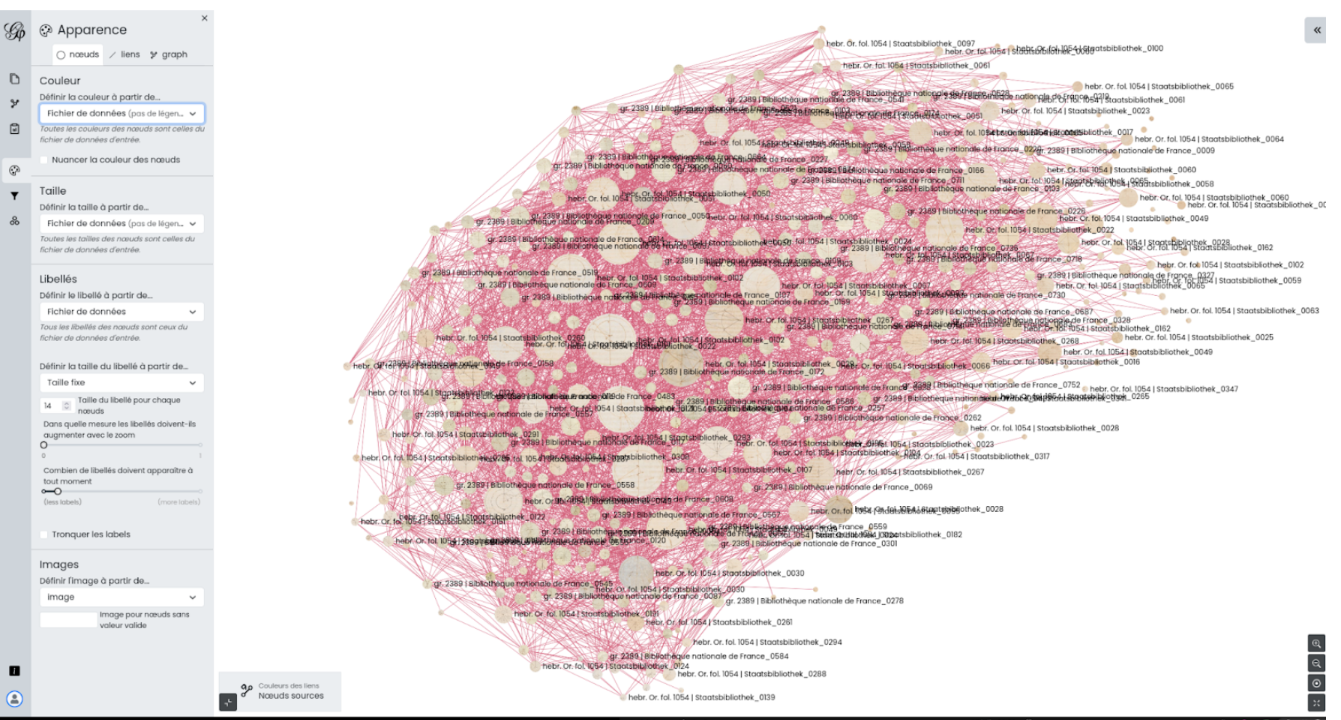
\includegraphics[width=1\textwidth]{images/visualisation_gephi_lite_2.png}
	\caption{Version finale de la visualisation \textit{Force-directed layout}}
	\label{fig:version_finale_gephi_lite}
\end{figure}

Comme nous pouvons le voir, la visualisation est plus aérée.

La visualisation \textit{bipartite graph} a aussi donné lieu à des retours de la part des chercheurs. Comme pour la \textit{Force-directed layout}, le nombre de relations posait problème pour la lisibilité et entraînait le plantage de la page. Pour y remédié, nous avons également supprimé les liens internes. Il a été aussi proposé de classer les \textit{regions} par page dans les différents \textit{witnesses} pour repérer l'endroit où elle se situe. 

\begin{figure}[H]
	\centering
	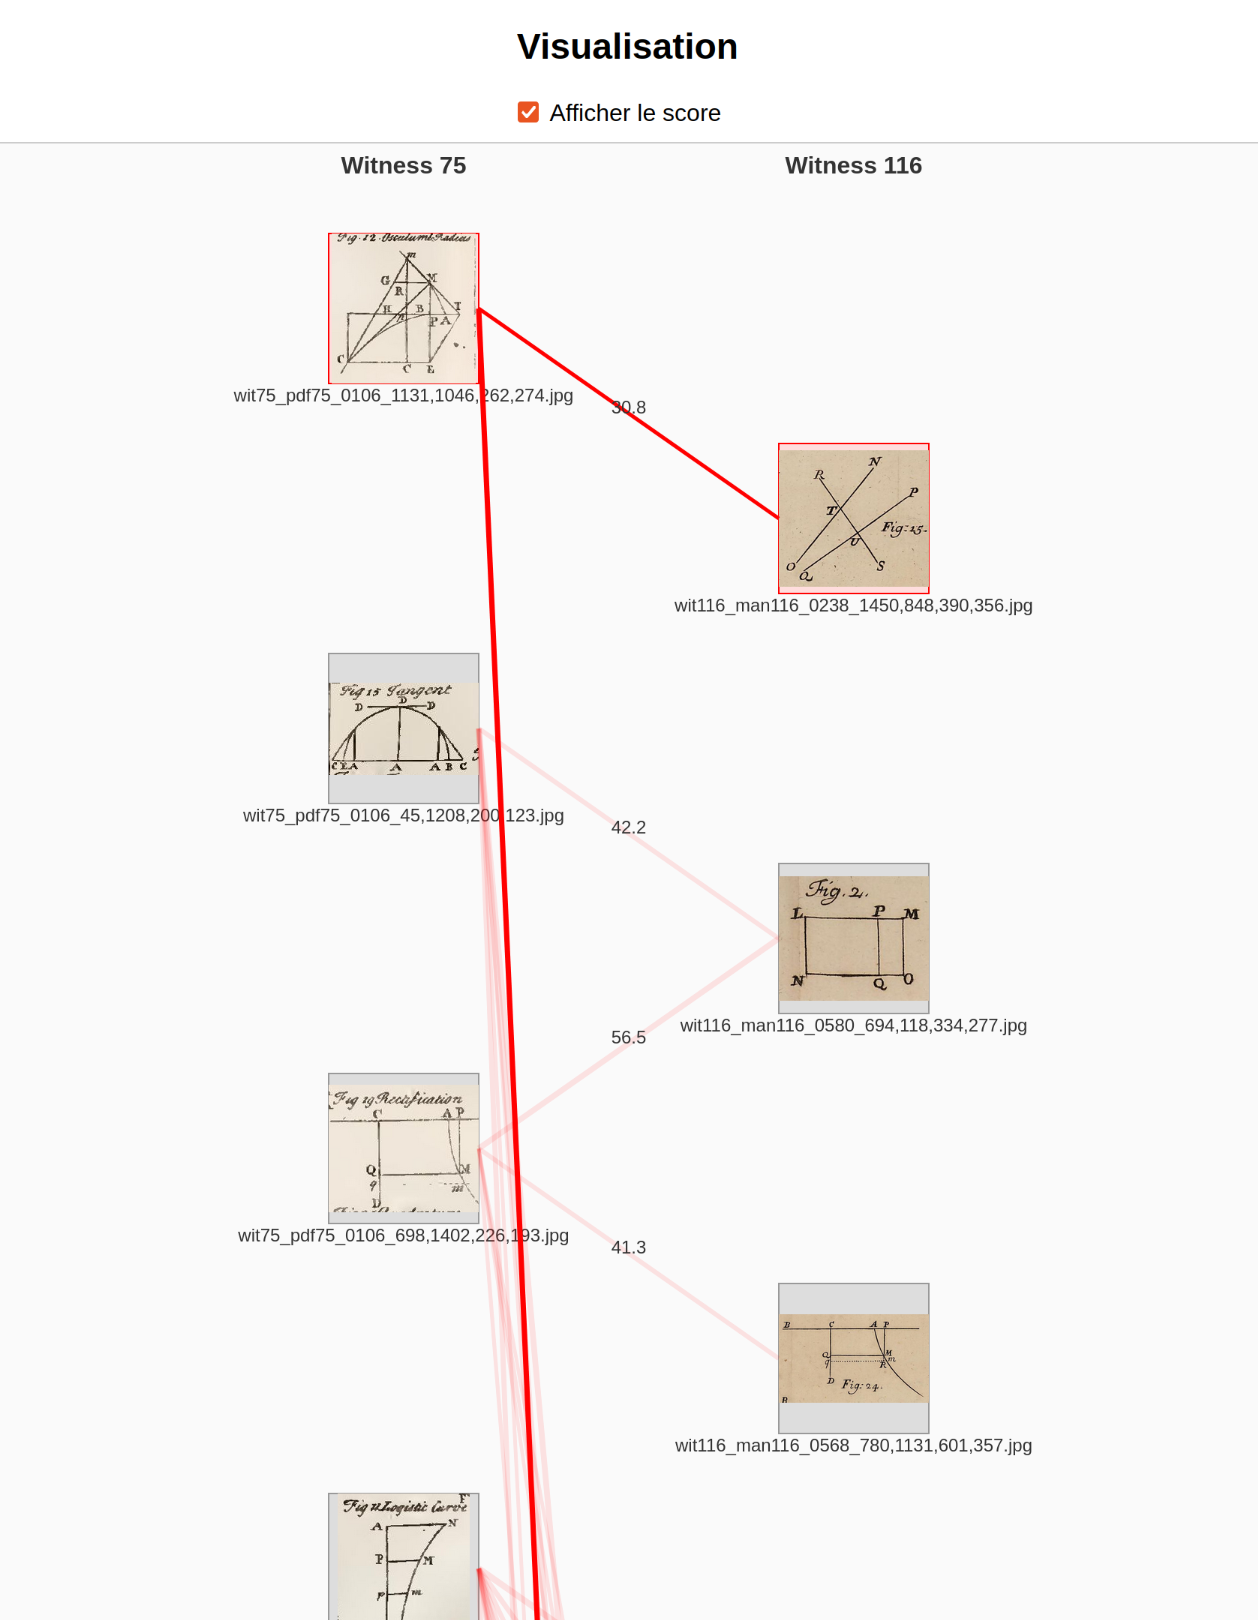
\includegraphics[width=1\textwidth]{images/version_finale_bipartite_graph.png}
	\caption{Version finale de la visualisation \textit{Bipartite-graph}}
	\label{fig:version_finale_bipartite}
\end{figure}

Une autre fonctionnalité a été évoquée : celle de développer un menu déroulant pour pouvoir choisir les \textit{witnesses} dont nous voulons comparer les \textit{regions}. Par exemple, dans notre cas, nous pourrions comparer les \textit{witnesses 75 et 116} puis les \textit{witnesses 76 et 116} sans avoir à changer la valeur de la variable \texttt{const file} dans le fichier \textit{index.html}.
 
